\documentclass{article}
\usepackage[utf8]{inputenc}
\usepackage{geometry}
 \geometry{
 a4paper,
 total={170mm,257mm},
 left=20mm,
 top=20mm,
 }
 \usepackage{graphicx}
 \usepackage{titling}

 \title{Module 5: Sonar
}
\author{Edvart Grüner Bjerke}
\date{November 2024}
 
 \usepackage{fancyhdr}
\fancypagestyle{plain}{%  the preset of fancyhdr 
    \fancyhf{} % clear all header and footer fields
    \fancyfoot[R]{
\includegraphics[width=2cm]{uio.png}}
    \fancyfoot[L]{\thedate}
    \fancyhead[L]{Module 5: Sonar}
    \fancyhead[R]{\theauthor}
}
\pagestyle{plain} % Apply the fancy style to all pages

\makeatletter
\def\@maketitle{%
  \newpage
  \null
  \vskip 1em%
  \begin{center}%
  \let \footnote \thanks
    {\LARGE \@title \par}%
    \vskip 1em%
    %{\large \@date}%
  \end{center}%
  \par
  \vskip 1em}
\makeatother

\usepackage{lipsum}  
\usepackage{subcaption}

\usepackage{cmbright}
\usepackage{amsmath}
\usepackage{array}
\usepackage{listings}
\usepackage{xcolor}

\lstdefinestyle{MatlabStyle}{
    language=Matlab,
    basicstyle=\ttfamily\small,        % Font size and family
    keywordstyle=\color{blue}\bfseries, % Color for keywords
    commentstyle=\color{green!50!black},% Color for comments
    stringstyle=\color{red},            % Color for strings
    backgroundcolor=\color{yellow!10},  % Background color for the code block
    frame=single,                       % Adds a frame around the code
    tabsize=4,                          % Tab size
    captionpos=b,                       % Position of the caption
    breaklines=true,                    % Automatic line breaking
    breakatwhitespace=true,             % Break at whitespace
    showspaces=false,                   % Don’t show spaces
    showstringspaces=false,             % Don’t show string spaces
}



\begin{document}

\maketitle


\subsection*{a)}
\begin{itemize}
    \item What is the theoretical angular resolution of the system at the center frequency?
\end{itemize}
To find the theoretical angular resolution we can use the following formula:
\[\delta \beta = \frac{\lambda}{L} \]
Where $\lambda$ is the wavelength and $L$ is the total array length
Given the number of elements $N_h$ with length $D$, the angular resolution becomes:

\[\delta \beta = \frac{\lambda}{N_h\cdot d} = \frac{0.0149m}{32*0.0375m} \]
\[\delta \beta = \underline{\underline{0.0124}}\]

\begin{itemize}
    \item What is the angular field of view of the system at the center frequency?
\end{itemize}

\noindent The field view (the beamwidth of the main lobe) is given by:
\begin{align}
    \beta \approx \frac{\lambda}{D} &= \frac{0.0149m}{0.0375m} = \underline{\underline{0.3973}} \\
\end{align}

\begin{itemize}
    \item What is the range (depth) resolution?
\end{itemize}

Given the assumed speed of sound in water $c$ and transmit bandwidth $B$, the range resolution is given by:


\begin{equation*}
    \begin{aligned}
        \delta r &= \dfrac{c}{2B} = \dfrac{1540 \ \text{m/s}}{2 \cdot 30,000 \ \text{s}^{-1}} \\
        &= 0.0257 \text{m} = \underline{\underline{25.67 \text{mm}}}
    \end{aligned}
\end{equation*}


\subsection*{b)}

\begin{itemize}
    \item Use Eq. (1) to generate a synthetic replica of the transmitted signal. Code must be presented.
\end{itemize}
To generate a replica of the transmitted signal, we consider the specified transmit equation:
\[ s_{Tx}(t) = \begin{cases} 
      \text{exp}(j2\pi\alpha t^2/2) & -T_p/2 \leq t \leq T_p/2 \\
      0 & |t| \ge T_p/2
   \end{cases}
\]
We first need to identify the parameters of the equation, and the number of samples to use in the array.
We initially only construct the non-zero part of the signal (though it's later padded for the FFT).
The number of transmit samples must be coherent with the time resolution used for the receive channel data. 
Otherwise, the convolution pulse compression implementation will give incorrect results. We 
can use the sampling frequency in the USTB object to determine the number of transmit samples:

\begin{lstlisting}[style=MatlabStyle]
alpha = (bw)/t_p;
n_transmit_samples = floor(t_p*channel_data.sampling_frequency);
t_transmit = linspace(-t_p/2, t_p/2, n_transmit_samples)';
s_Tx = exp(j*2*pi*alpha*t_transmit.^2/2);
\end{lstlisting}

\newpage
\begin{itemize}
    \item Implement a pulse compression algorithm in MATLAB.
\end{itemize}

\noindent For the implementation of pulse compression, we use the Fourier Transform formulation:
\[s_m(\tau) = \mathcal{FT}^{-1}\left\{\mathcal{FT}\left\{s_{Rx}(t)\right\}\mathcal{FT}\left\{s_{Tx}(t)\right\}^* \right\} \]

\noindent The empty result buffer is created, with twice the length of the original signal. This is necessary, since
the convolution operation (done here through the FFT) doubles the length as the two signals "pass through" each other:

\lstset{language=Matlab}
\begin{lstlisting}[style=MatlabStyle]
match_filtered_data = zeros(2*n_receive_samples-1, channel_data.N_elements);
\end{lstlisting}

\noindent Then, for each array element, we perform the pulse compression using the fast fourier transform.
The received channel data is extracted, and the FFT is performed on the receive and transmit data. The number of samples \verb|n| is 
set equal to the result length, which pads the data. Finally, we take the inverse fourier transform of the 
transformed receive data multiplied by the complex conjugate of the transformed transmit data. 
We also make sure to only store the first \verb|n_receive_samples| elements of the result into the USTB object:

\begin{lstlisting}[style=MatlabStyle]
for elem = 1:channel_data.N_elements
    s_Rx = channel_data.data(:, elem);
    % Do FFT compression
    S_Rx = fft(s_Rx, 2 * n_receive_samples - 1);
    S_Tx = fft(s_Tx, 2 * n_receive_samples - 1);
    s_m = ifft(S_Rx .* conj(S_Tx));
    match_filtered_data(:, elem) = s_m;
end
channel_data_compressed.data = match_filtered_data(1:n_receive_samples, :);
\end{lstlisting}


\begin{itemize}
    \item Describe the difference between the raw data and the pulse compressed data. Explain why there is a
    difference.
\end{itemize}

\noindent From the figure, we can see that the matched filter (pulse compression) significantly reduces the noise in the signal.
This is possible because we know the exact (theoretical) transmitted pulse, which is used by the matched filter. 
Conceptually, the filter tries to identify (or "match") the transmit signal in the received signal by performing a convolution.
This way we can filter out parts of the receive signal that are not related to the transmitted signal.
The result is a signal with maximum Signal-to-Noise Ratio (given additive white gaussian noise).

\begin{figure}[h]
    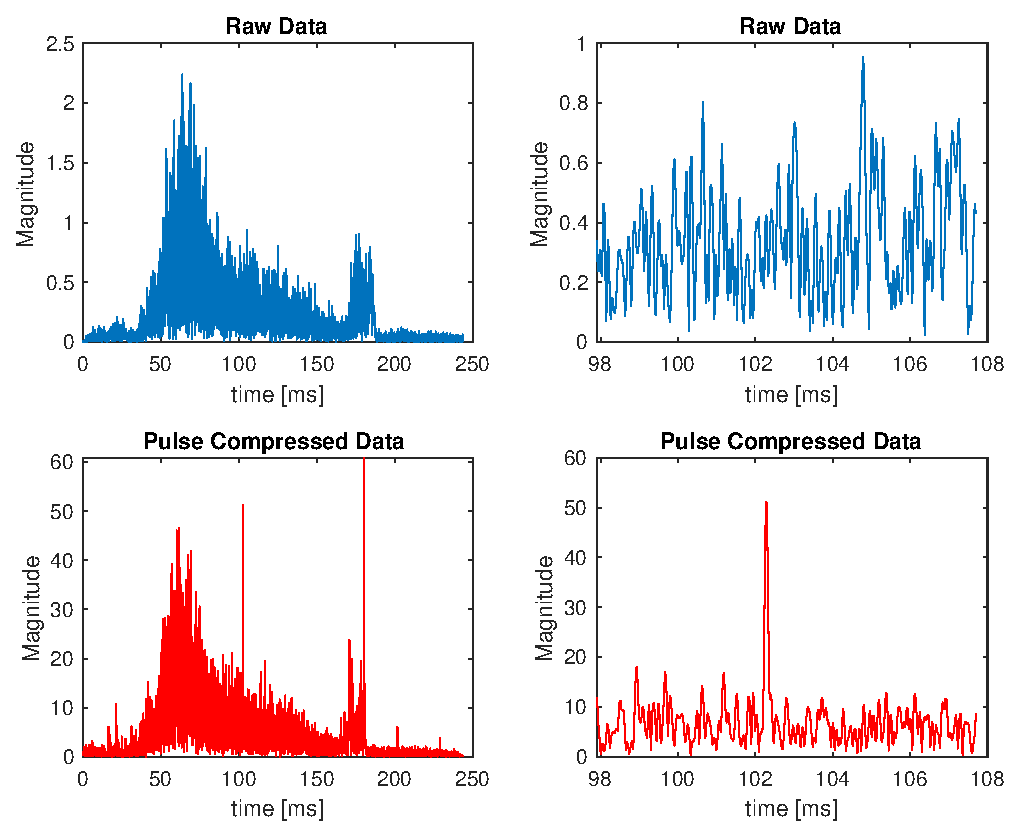
\includegraphics[width=10cm]{epsFig}
    \centering
    \caption{The result of pulse compression on a single channel}
\end{figure}


\newpage
\subsection*{c)}
\begin{itemize}
    \item Define the image scan
\end{itemize}

\noindent Here, we define a simple sector scan using the parameters found in a):
\begin{lstlisting}[style=MatlabStyle]
az_res = 0.0124;
range_res = 0.02566;
scan = uff.sector_scan();
scan.depth_axis = [0:range_res:160];
scan.azimuth_axis = [-0.2:0.0124:0.2];    
\end{lstlisting}

\begin{itemize}
    \item Run the processing object on both channel data objects.
\end{itemize}
We set up a delay-and-sum pipeline in USTB and perform beamforming without receive or transmit apodization:
\begin{lstlisting}[style=MatlabStyle]
    az_res = 0.0124;
    range_res = 0.02566;
    scan = uff.sector_scan();
    scan.depth_axis = [0:range_res:160];
    scan.azimuth_axis = [-0.2:0.0124:0.2];    
    \end{lstlisting}

\begin{itemize}
    \item Run the processing object on both channel data objects
\end{itemize}

\noindent We build and run a midprocess USTB pipeline and simply swap the channel data for the raw/compressed signals:
\begin{lstlisting}[style=MatlabStyle]
mid = midprocess.das();
mid.scan = scan;
mid.transmit_apodization.window=uff.window.none;
mid.receive_apodization.window=uff.window.none;
mid.code = 'matlab';
mid.channel_data = channel_data;
% beamform raw data
b_data = mid.go();
% beamform pulse compressed data
mid.channel_data = channel_data_compressed;
b_data_compressed = mid.go();
\end{lstlisting}

\newpage

\begin{itemize}
    \item Display the results
\end{itemize}

\noindent We first show the final result of beamforming on the raw and pulse compressed channel data:

\begin{figure}[ht]
    \centering
    % First subfigure
    \begin{subfigure}{0.3\textwidth} % Adjust width as necessary
        \centering
        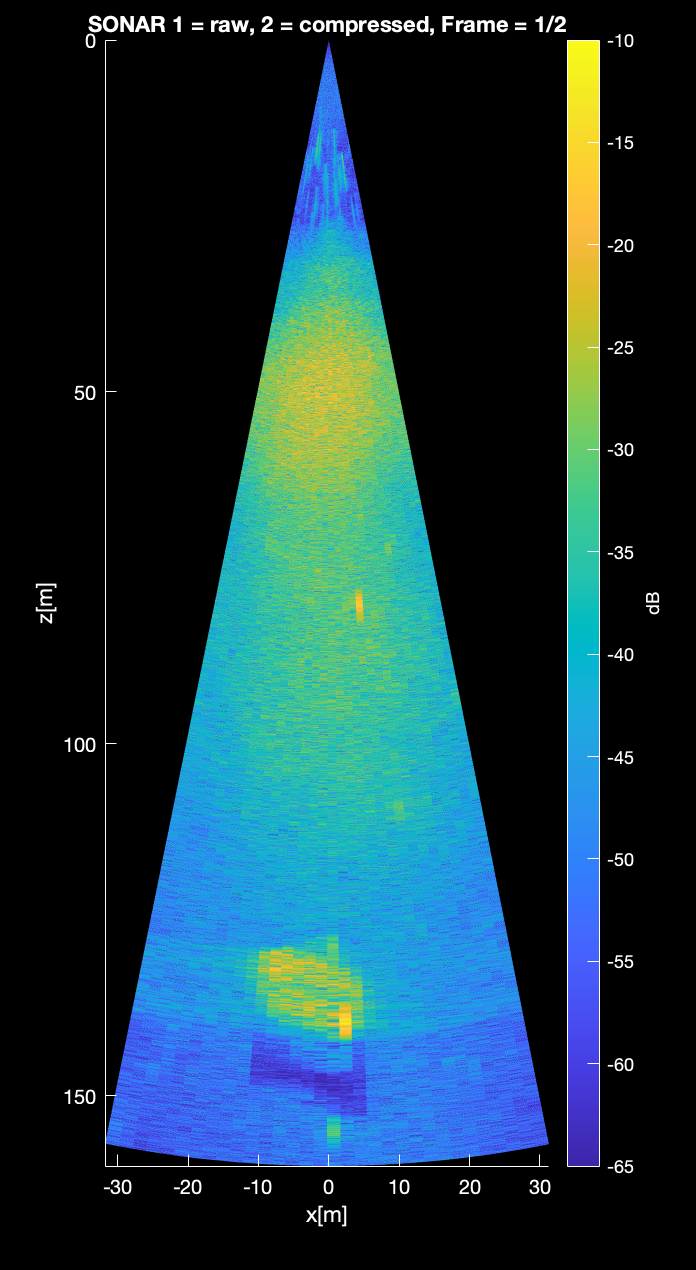
\includegraphics[width=\linewidth]{b_raw.png} % Replace with your image file
        \caption{Raw beamformed image}
        \label{fig:sub1}
    \end{subfigure}
    \hspace{0.05\textwidth}
    \begin{subfigure}{0.3\textwidth} % Adjust width as necessary
        \centering
        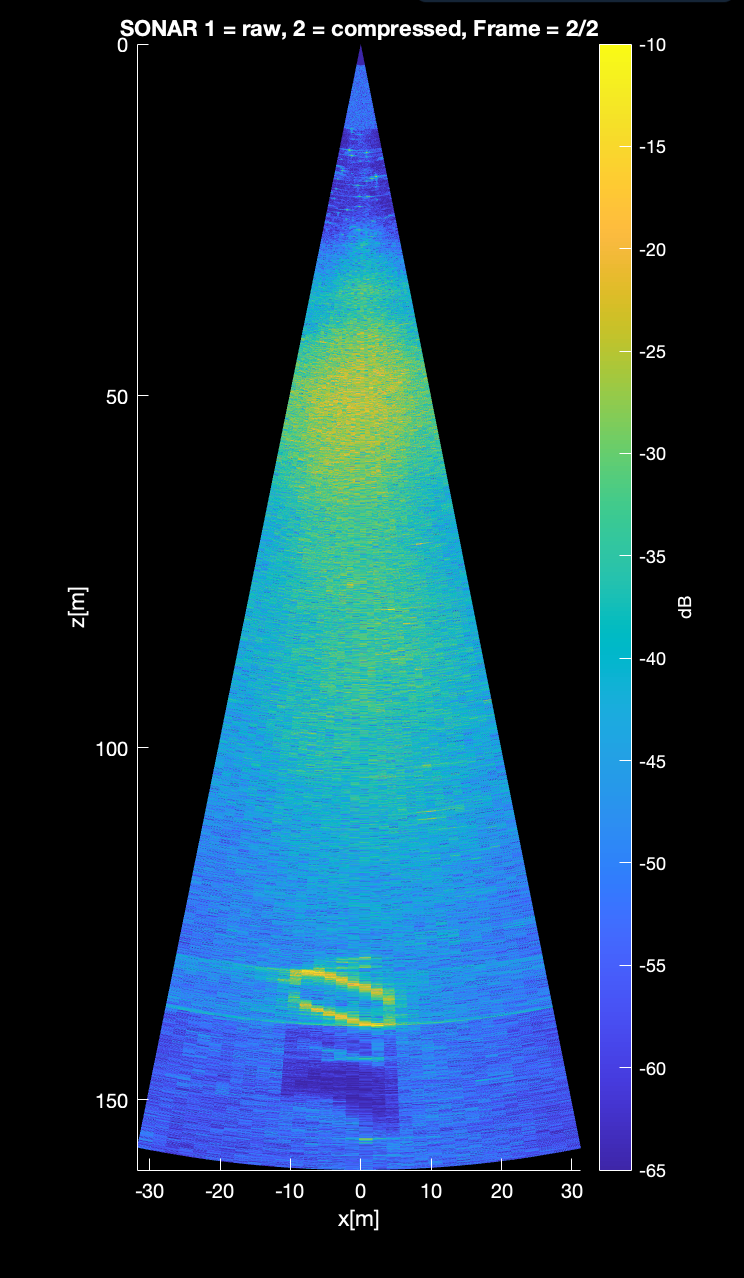
\includegraphics[width=\linewidth]{b_compressed.png} % Replace with your image file
        \caption{Pulse compressed beamformed image}
        \label{fig:sub2}
    \end{subfigure}
    \label{fig:main}
\end{figure}

We see a clear improvement in SNR and contrast, and the contour of the object of interest is much clearer. In general, we also see a reduction in the ambient noise in the image.


To visualize the data before beamforming (raw and compressed), we can zoom into an area of interest. Here
we have zoomed in on the object appearing in the scan. From the figure, we can see that the pulse compressed channel data
is more distinct, with clearly defined borders:


\begin{figure}[ht]
    \centering
    % First subfigure
    \begin{subfigure}{0.3\textwidth} % Adjust width as necessary
        \centering
        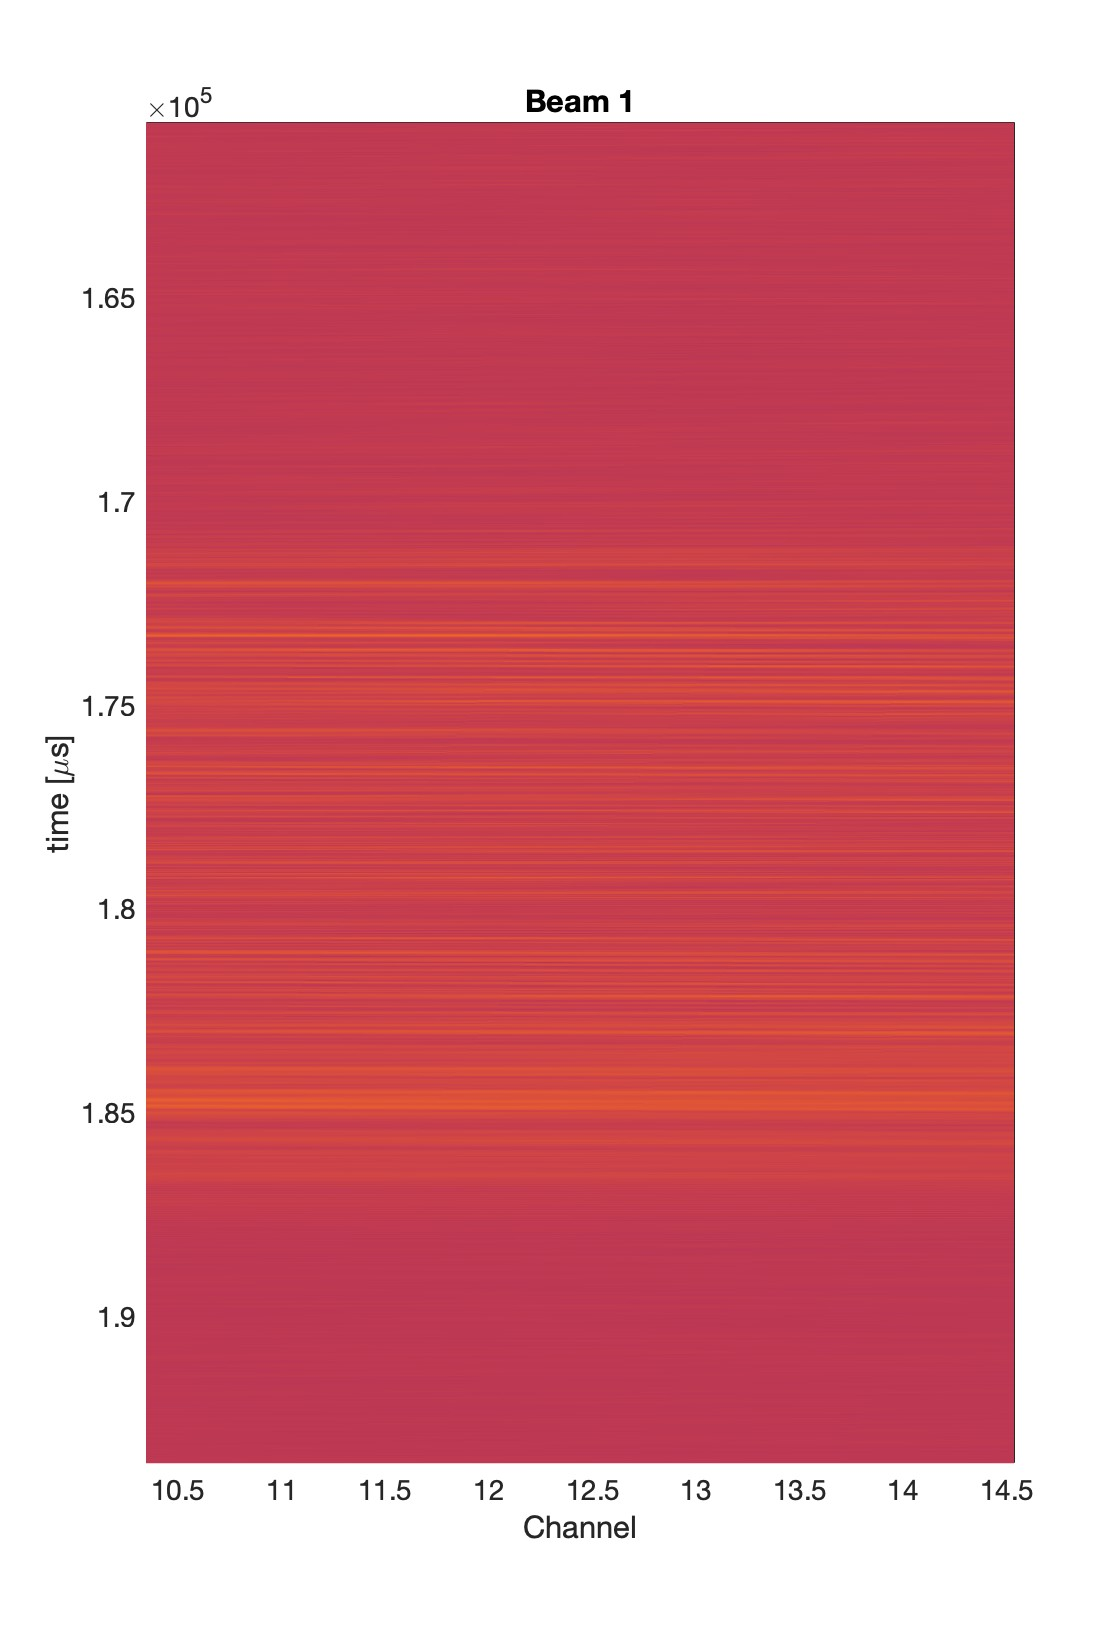
\includegraphics[width=\linewidth]{raw.jpg} % Replace with your image file
        \caption{Raw channel signals}
        \label{fig:sub1}
    \end{subfigure}
    \hspace{0.05\textwidth}
    \begin{subfigure}{0.3\textwidth} % Adjust width as necessary
        \centering
        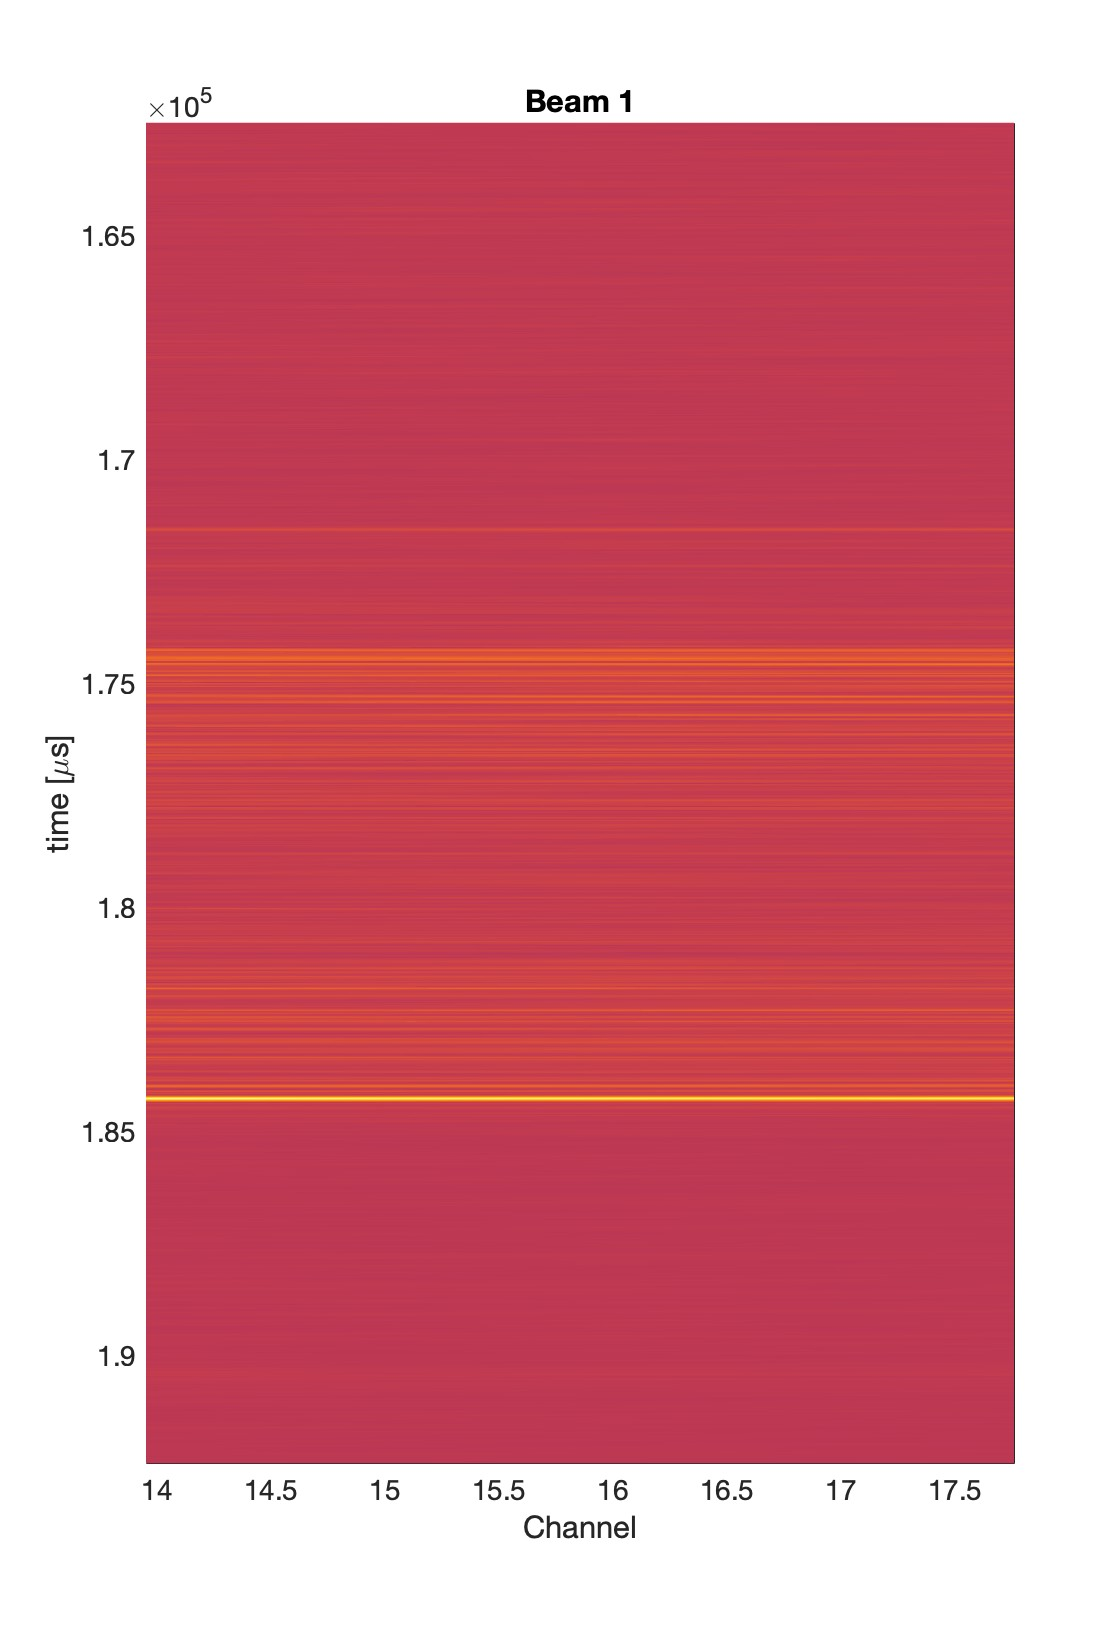
\includegraphics[width=\linewidth]{compressed.jpg} % Replace with your image file
        \caption{Pulse compressed channel signals}
        \label{fig:sub2}
    \end{subfigure}
    \label{fig:main}
\end{figure}


\begin{itemize}
    \item There is a target at approximately 130 m range. What is it? How large is it in meters?
\end{itemize}

We can measure the approximate size of the object by looking directly at the plot, since the axes are in meters.
\[\text{L} \approx 14.7\text{m}\]
\[\text{D} \approx 8.0\text{m}\]
I'm not quite sure what the object is. Maybe it is a boat? :)

\end{document}
